\documentclass{article}
\usepackage[utf8]{inputenc}
\usepackage{graphicx}
\usepackage{amsmath}
\documentclass[10pt,a4paper]{article}
\usepackage{geometry}



\begin{document}

%Set Title
\title{Stochastic Assignment  2 \\ Wiener Filter}
\author{Hanna Nabil}
\maketitle

\section{Introduction}
In signal processing, the Wiener filter is a filter used to produce an estimate of a desired or target random process by linear time-invariant (LTI) filtering of an observed noisy process, assuming known stationary signal and noise spectra, and additive noise. The Wiener filter minimizes the mean square error between the estimated random process and the desired process.
\section{Description}

The goal of the Wiener filter is to compute a statistical estimate of an unknown signal using a related signal as an input and filtering that known signal to produce the estimate as an output. For example, the known signal might consist of an unknown signal of interest that has been corrupted by additive noise. The Wiener filter can be used to filter out the noise from the corrupted signal to provide an estimate of the underlying signal of interest. The Wiener filter is based on a statistical approach, and a more statistical account of the theory is given in the minimum mean square error (MMSE) estimator article.

Typical deterministic filters are designed for a desired frequency response. However, the design of the Wiener filter takes a different approach. One is assumed to have knowledge of the spectral properties of the original signal and the noise, and one seeks the linear time-invariant filter whose output would come as close to the original signal as possible. 


\section{Problem Formulation}
We have Given a distorted ECG signal. We have modelled the distortion as  follow

\centerline{$y(n) = cx(n) + v(n)$}          
where y(n) is the distorted signal. x(n) is the source signal, and v(n) is WGN v(n) \sim N (0, $\sigma ^{2})$ 
 $c = -3 $   and $\sigma_v ^{2}$ = 0.02
\begin{description}

\item [$\bullet$ ] Using provided model, build a third order Wiener filter.
\item [$\bullet$ ]  Apply this filter on the signal and show the  output.
\item [$\bullet$ ] Calculate mean square error of filtered signal (Source signal is provided for that).

\end{description}
 


\section{Implementation}
First we get the Zero Mean of the distorted Signal Y (Subtract it from the mean)
Then we get correlation Matrix $Ryy$  we can get it from numpy.correlate in Python or implement it manually actually I preferred to implement it manually 
after that we got an array of the same size as $Y$ (the distorted Signal ) actually we need only 3 elements of that array according to the filter Order which is 3 
After that we get the Filter Coefficients From this Formula


\begin{equation}
\begin{bmatrix} h(0)\\ h(1)\\  h(2) \end{bmatrix}
=\frac{1}{c}
\begin{bmatrix}
R_{yy}(0) & R_{yy}(1) & R_{yy}(2)\\
R_{yy}(1) & R_{yy}(0) & R_{yy}(1)\\
R_{yy}(2) & R_{yy}(1) & R_{yy}(0) 
\end{bmatrix}^{-1}
\begin{bmatrix}
R_{yy}(0) -\sigma_{v}^2 \\
R_{yy}(1) \\
R_{yy}(2)  
\end{bmatrix}
\end{equation}

\section{Sample Results}
\subsection{Filtered VS Distorted Signals}

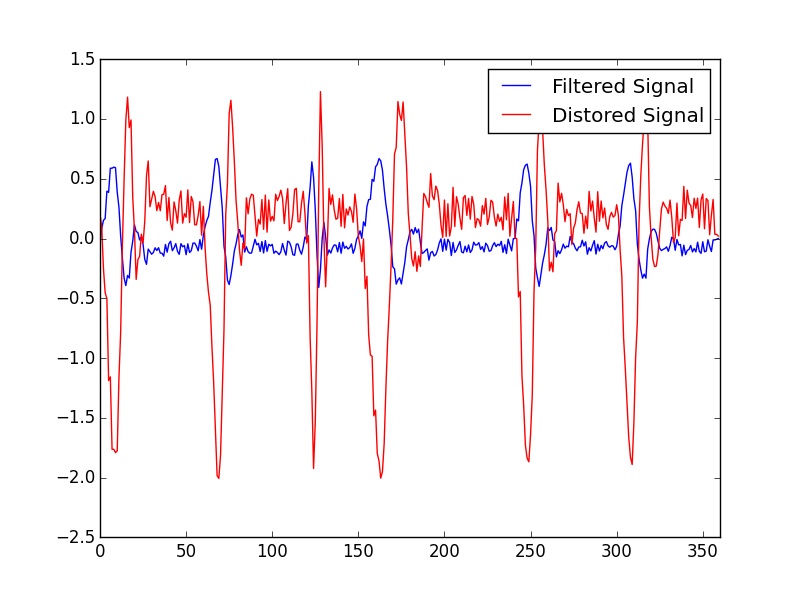
\includegraphics[scale=0.8]{filtered_and_distorted_signals.png}
\subsection{Original VS Filtered Signals}

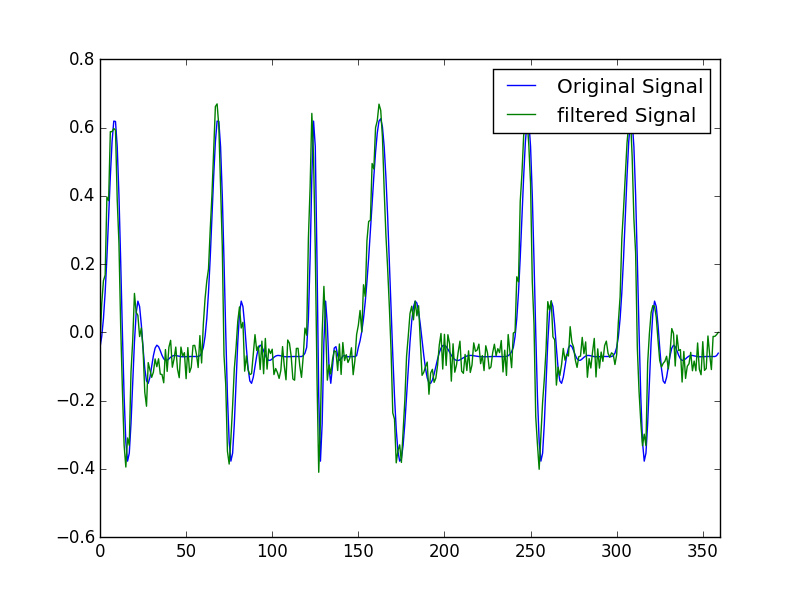
\includegraphics[scale=0.8]{original_vs_filtered.png}

\end{document}
